\chapter{Basic CNN}

This model is a specialized kind of neural network for processing data that has a known, grid-like topology, or more generally, data $X^i \in \mathbb{R}^{n_1\times n_2\cdots\times n_d}$ is a order $d$ tensor. A naive way to deal with those kind of data is to reshape this tensor to be a vector( order 1 tensor), and then use the traditional deep feedforward neural network.

However, for some practical problem, this method means that the input dimension is very big that is $m = n_1\times\cdots \times n_d$. Another important reason is that this will broke the structure of this data, especially for AI task.

\section{Convolution in mathematics}
\subsection{Continuous case}
Generally speaking, convolution is a special kind of bilinear transform for multidimensional function. For example:
\begin{equation}
\ast: L^2(\mathbb{R}^n) \times L^2(\mathbb{R}^n) \to L^1(\mathbb{R}^n).
\end{equation}

So if, we fixed one function, a convolution operator is just a linear transform form one function space to another. For example, if $g \in C_0^{\infty}(\mathbb{R}^n)$, we have:
\begin{equation}
\ast g: L^2(\mathbb{R}^n) \to L^2(\mathbb{R}^n),
\end{equation}
with 
\begin{equation}
(f\ast g)(x) := ((\ast g)f )(x) = \int_{\mathbb{R}^n} f(y)g(x-y) dy. 
\end{equation}

\subsection{Discrete case}
When talks about discrete case, general function becomes tensor(Although, the real tensor definition is not like this):
Functions $\to$ Tensors, 
\begin{align}
(f\ast g)(x) &= \int_{\bm{y}} f(x_1 - y_1,\cdots,x_d - y_d)g(y_1,\cdots,y_d) \\
\xrightarrow[Uniform~Grid]{Sampling} (F\ast G)_{i_1, \cdots, i_d} &= \sum_j F_{i_1 - j_1,\cdots,i_d - j_d}G_{j_1, \cdots, j_d}.
\end{align}


We can have the next definition for two general order $d$ tensor(comes from the $d$-dimensional function):
\begin{equation}
(T\ast M)(i_1, i_2, \cdots ,i_d) = \sum_{j_i, j_2,\cdots,j_d \in \mathbb{Z}} T(j_1, j_2,\cdots,j_d)M(i_1 - j_1, i_2 - j_2, \cdots, i_d - j_d).
\end{equation}
Almost book and notes about CNN defined discrete convolution like this, but here is a problem about the summation  index, this may only be well defined when the index for every dimension can be infinite. So in general there should be some rules for finite cases, for example: 
\begin{itemize}
\item Padding $M$ with zeros
\item Repeat $M$ to make it a periodic infinite one in every dimension
\end{itemize}
Now we consider the finite case, which means $T, M \in \mathbb{R}^{n_1 \times n_2 \times \cdots n_d}$. By the definition(no matter what rules we use), $\ast M$ should be a order $2d$ tensor with some special structure because that:
\begin{equation}
\ast M \in L(\mathbb{R}^{n_1 \times n_2 \times \cdots n_d}, \mathbb{R}^{n_1 \times n_2 \times \cdots n_d}).
\end{equation}
And we call $M$ is the kernel for this convolution mapping $\ast M$.

Here a good example for the special structure for $\ast M$ is when we consider the convolution between two order $1$ tensors. We can have two vectors $\bm{x}$ and $\bm y$ then $\ast \bm y$ is exact the a special Toeplitz matrix i.e a circulant matrix. 
\begin{equation}
(\ast \bm{y})_{i,j} = \bm{y}(j-i+1).
\end{equation}
We will see that, this special structure plays a very important role in deep learning, I think this special structure is a special case for general called ``Parameter Sharing".  



\section{Convolution introduction in CNN (without multichannel)}
\subsection{General Convolution in CNN(with small size change)}
There is a kind of special linear map from some general finite dimension tensor space to another is called ``convolution".  Generally, we have a tensor like $X \in \mathbb{R}^{n \times m}$ and a small kernel such as $K \in \mathbb{R}^{k\times k}$, then we have:
\begin{definition}[Original Convolution with stride 1 for CNN]
\begin{equation}\label{equ:conv}
(X\ast K)_{i,j} = \sum_{s, t = 1}^k X_{i-1 + s, j-1 + t} K_{s,t}.
\end{equation}
It's easy to see that $(X\ast K) \in \mathbb{R}^{(n-k + 1) \times (m-k + 1)}$.
\end{definition}
If we use stride $p$, we have:
\begin{definition}[Original Convolution with stride $p$ for CNN]
\begin{equation}\label{equ:convstride}
(X\ast_{p} K)_{i,j} = \sum_{s, t = 1}^k X_{(i-1)p + s, (j-1)p + t} K_{s,t}.
\end{equation}
So, we have 
$
(X\ast_p K) \in \mathbb{R}^{((n-k)/p + 1) \times ((m-k)/p+1)}.
$
\end{definition}
This stride properties in some application are often used as pooling(subsampling, coarsening).  

Here we can define a special pooling operator as $S^p$ which likes the $C/F$ split for choosing coarse point:
\begin{equation}
S^p(X)_{i,j} = X_{(i-1)p + 1, (j-1)p + 1},
\end{equation}
then we have:
\begin{equation}\label{equ:stride}
X \ast_p K = S^p(X\ast K),
\end{equation}
with the $\ast$ and $\ast_p$ defined by \ref{equ:conv} and \ref{equ:convstride}
\begin{proof}
\begin{align}
S^p(X \ast K)_{i,j} &= (X \ast K)_{(i-1)p+1, (j-1)p + 1}  \\
&= \sum_{s,t = 1}^k X_{(i-1)p + 1 -1 +s, (j-1)p +1 -1 +t}K_{s,t}  \\
&= (X \ast_p K)_{i,j}.
\end{align}
\end{proof}

\subsection{Convolution with Padding in CNN(without changing size)}
For many case kernel size is some small odd numbers such as 1, 3, 5... So we ca have those next definition for convolution:
\begin{definition}[Convolution with Padding]

We write $K\in \mathbb R^{2k+1, 2k+1}$, we then write
\begin{equation}\label{ConvPadding}
(X \ast K)_{i,j} :=\sum_{s, t = -k}^k P^k(X)_{i + s, j + t} K_{s,t},
\end{equation}
with $\rm{P}^k$ means Padding. 
\end{definition}
Here we see that, to make this definition well-defined, we have $X\ast K \in \mathbb{R}^{n-2k, m-2k}$, because if the index of $X$ start from $1$ to $n(m)$, then $X \ast K$ from $k+1$ to $n(m) - k$. To make the convolution don't change size, we can use Padding strategy like in image process. 
%In fact, if the resolution is very high, which means the measure of the boundary of the image is close to 0, so in traditional image process, this strategy hasn't been studied very well. There are basic three strategy:
\begin{description}
\item[Zero Padding] The simplest and most common used strategy is zero padding with:
\begin{equation}
\rm{P}^k_0: \mathbb{R}^{n \times m} \to \mathbb{R}^{n+2k \times m+2k}
\end{equation}
with 
\begin{equation}
\rm{P}_0^k(X)_{i,j} = \begin{cases}
0 &i(j)=-k+1:0 ~~\text{and}~~ i(j) = n(m)+1:n(m)+k \\
X_{i,j} &i(j) = 1:n(m) 
\end{cases}
\end{equation}
\item[Reflection Padding] This strategy is defined by:
\begin{equation}
\rm{P}^k_r: \mathbb{R}^{n \times m} \to \mathbb{R}^{n+2k \times m+2k}
\end{equation}
with 
\begin{equation}
\rm{P}_r^k(X)_{i,j} = \begin{cases}
X_{1-i, 1-j} &i(j)=-k+1:0 ~~\text{and}~~ i(j) = n(m)+1:n(m)+k \\
X_{i,j} &i(j) = 1:n(m) \\
0 &\text{others} 
\end{cases}
\end{equation}
\item[Shift Padding] This strategy is defined by:
\begin{equation}
\rm{P}^k_s: \mathbb{R}^{n \times m} \to \mathbb{R}^{n+2k \times m+2k}
\end{equation}
with 
\begin{equation}
\rm{P}_s^k(X)_{i,j} = \begin{cases}
X_{k-i, k-j} &i(j)=-k+1:0 ~~\text{and}~~ i(j) = n(m)+1:n(m)+k \\
X_{i,j} &i(j) = 1:n(m) \\
0 &\text{others} 
\end{cases}
\end{equation}
\end{description}

So we can have:
\begin{equation}
\rm{dim}(X\hat{\ast}K) = \rm{dim}(\rm{P}^k(X) \ast K) = \rm{dim}(X),
\end{equation}
and the $i,j$ index is consistent for both side of the above equation where $\rm{P}^k = \rm{P}_0^k, \rm{P}_{r}^k$ or $\rm{P}_s^k$.


\begin{remark}We note all the later convolution as the \eqref{ConvPadding} without special statements and use $\ast$ stands for $\hat{\ast}$.

\end{remark}



\section{Special Structure for Convolution in CNN}
Now let us forget about the general convolution in mathematics, we go back to the method for using deep learning to deal with tensor data. Recall the general method in fully connected deep feedforward neural network, all process can be decompose into two phase: linear transform(in fact, affine map) from vector space to another vector space,  and nonlinear transform separately for every component for the output of linear transform. 

So, now we consider we have a tensor like $T \in \mathbb{R}^{n_1\times n_2\cdots \times n_d}$, and we want to use some linear transform $W$ such that $W(T) \in  \mathbb{R}^{n'_1\times n'_2\cdots \times n'_d }$, this means that 
\begin{equation}
W \in  L(\mathbb{R}^{n_1\times n_2\cdots \times n_d},  \mathbb{R}^{n'_1\times n'_2\cdots \times n'_{d}}) ,
\end{equation}
which means that $W$ is a order $2d$ tensor. The size for $W$ is too big!

\subsubsection{Parameter Sharing and Convolution}
Let us just use the order 1 tensor as a example to show the power for parameter sharing. For vector case, i.e $T \in \mathbb{R}^{n}$, and we want the output is in $\mathbb{R}^m$, so we have $W \in R^{m\times n}$.  So we can think about the next parameter sharing strategy:
\begin{definition}[Parameter Sharing]
Every row of $W$ is same without only some shifting operator.  
\end{definition}
This strategy lead to that the convolution operator is a very special kind of  result from parameter sharing.  This means that $W$ can be defined by just a $\mathbb{R}^n$ vector.(This might be some kinds of ``low dimension" structure?) However, how to choose a suitable vector is still a big problem. By the way, for general tensor, this means that $W$ also have the same size for $T$ which may also be a little big.  

\subsubsection{Sparsity for Convolution in CNN}
Thanks for the filter theory for mathematical image process, we can just choose some sparse(local supported) vector to do some meaningful operation. Such as   $(-1, 2, -1)$, means the discrete Laplacian operator, but a more strict expression should be $\bm x \in \mathbb{R}^n$, and then $W \in \mathbb{R}^{n-2 \times n}$ with 
\begin{equation}
W(j,i) = w(j - i + 1)  \quad  W = \begin{pmatrix}
-1 & 2 & -1 & 0 & 0&\cdots & 0 \\
0& -1 & 2 & -1 & 0 & \cdots & 0 \\
\vdots &  & & \cdots & & & \vdots \\
0& \cdots & & & -1 & 2& -1 
\end{pmatrix},
\end{equation}
and 
\begin{align}
\bm x\ast w = W \bm x.
\end{align}
So we may have the next with sparse parameter strategy:
\begin{definition}[Sparsity]
Every row of $W(:,i)$ is locally supported around $i$ or $i \pm 1$.  
\end{definition}

At last, we can take this kind of convolution in CNN as a results of ``parameter sharing" and ``sparsity". 

%\subsection{Convolution in CNN}
%\subsubsection{Definition by ``inner product" type operator}
%For the example above, we found that we only need a vector $ k = (-1,2,-1)$ to represent this process like:
%\begin{equation}
%(W \bm x)(j) = x(j:j+2) \cdot k \quad \forall j = 1:n-2.
%\end{equation} 
%So this inspires us to have the next definition, if $T \in \mathbb{R}^{n_1 \times n_2 \cdots n_d}$ and $K \in \mathbb{K}^{m_1 \times m_2\cdots m_d}$ with $ m_i \le n_i $. 
%we can define 
%\begin{equation}
%\hat{m}_i = \begin{cases}
%\frac{m_i - 1}{2} \quad &\text{if $m_i$ is odd} \\
%\frac{m_i}{2} \quad &\text{if $m_i$ is even}.
%\end{cases}
%\end{equation}
%So we define 
%\begin{equation}
%(T \ast K)(i_1, i_2, \cdots, i_d) = T( i_1 : i_1 + (m_i-1), \cdots, i_d:i_d + (m_d -1)) \odot K \quad i_j \le n_j - m_j + 1,
%\end{equation}
%where $\odot$ means sum of all index for two tensor with the same size, i.e 
%\begin{equation}
%T_1 \odot T_2 = \sum_{i_1, \cdots, i_d} T_1(i_1, \cdot, i_d) T_2(i_i,\cdots, i_d).
%\end{equation}
%This means that, for any tensor we can use another tensor with the same order and smaller size to be a kernel, and do convolution with them. So this is no longer commutative for this kind of ``convolution".


\subsection{Convolution with multichannel}
\subsubsection{Channel}
Before we start to explain every layers for general CNN model, we want to give some remarks about ``Channel".   As we know above, if we apply one certain kernel to do convolution with the original tensor, we can get some certain feature. The following are some examples of $3\times 3$ kernels.
%\begin{figure}[!htb]        
	%\center{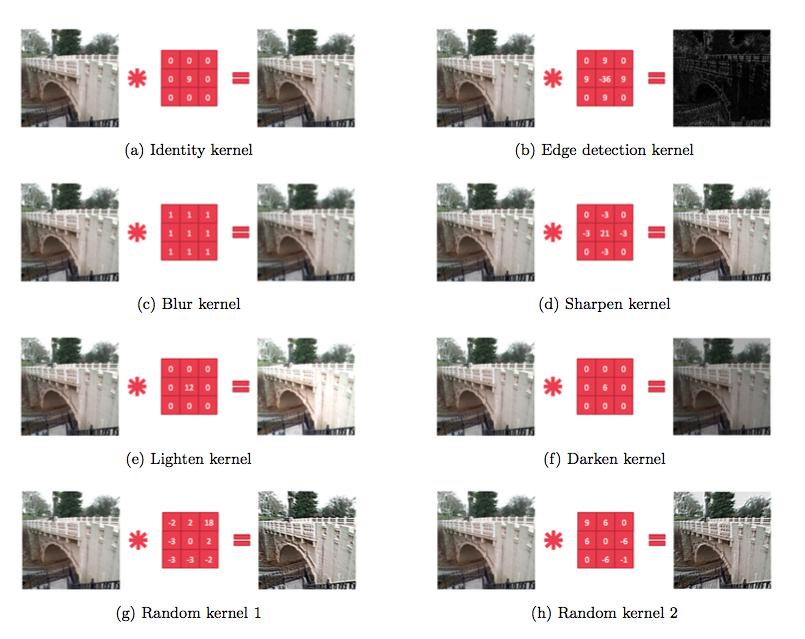
\includegraphics[width=13cm] {Kernels.png}}        
	%\caption{Eight kernels makes eight channels with different type of features.}      
	%\label{Kernels}
%\end{figure}
\begin{itemize}
\item A horizontal bar 
$$
\raisebox{-.5\height}{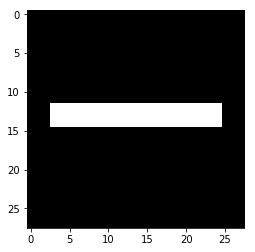
\includegraphics[width=0.2\textwidth]{horizontal.png}} *
\begin{pmatrix}
    0 & 0 & 0\\
    0 & 1 & 0\\
    0 & 0 & 0
\end{pmatrix} = 
\raisebox{-.5\height}{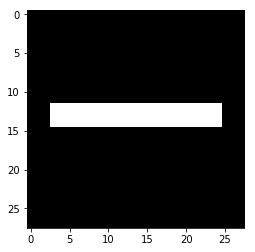
\includegraphics[width=0.2\textwidth]{horizontal.png}} 
$$
$$
\raisebox{-.5\height}{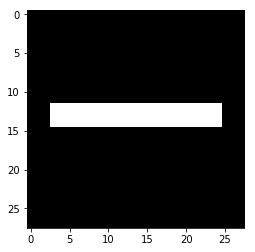
\includegraphics[width=0.2\textwidth]{horizontal.png}} *
\begin{pmatrix}
    1 & -1 & 0\\
    0 & 0 & 0\\
    0 & 0 & 0
\end{pmatrix} = 
\raisebox{-.5\height}{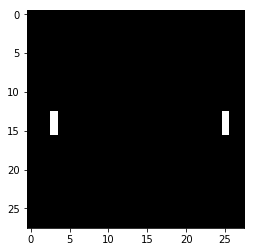
\includegraphics[width=0.2\textwidth]{hx.png}} 
$$
$$
\raisebox{-.5\height}{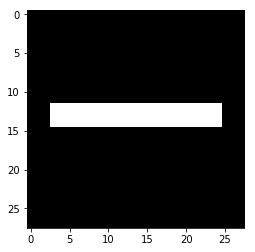
\includegraphics[width=0.2\textwidth]{horizontal.png}} *
\begin{pmatrix}
    1 & 0 & 0\\
    -1 & 0 & 0\\
    0 & 0 & 0
\end{pmatrix} = 
\raisebox{-.5\height}{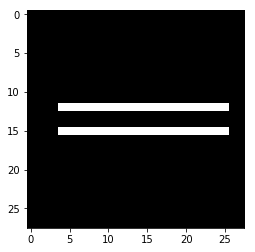
\includegraphics[width=0.2\textwidth]{hy.png}} 
$$
$$
\raisebox{-.5\height}{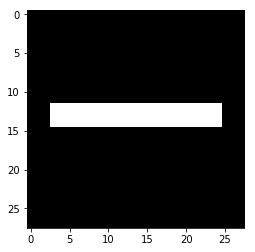
\includegraphics[width=0.2\textwidth]{horizontal.png}} *
\begin{pmatrix}
    -1 & 0 & 0\\
    0 & 1 & 0\\
    0 & 0 & 0
\end{pmatrix} = 
\raisebox{-.5\height}{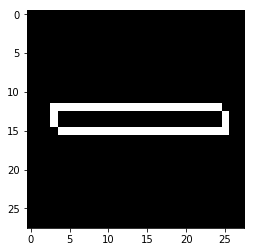
\includegraphics[width=0.2\textwidth]{hxy.png}} 
$$
$$
\raisebox{-.5\height}{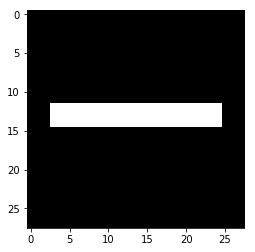
\includegraphics[width=0.2\textwidth]{horizontal.png}} *
\begin{pmatrix}
    0 & -1 & 0\\
    -1 & 4 & -1\\
    0 & -1 & 0
\end{pmatrix} = 
\raisebox{-.5\height}{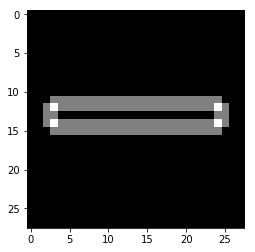
\includegraphics[width=0.2\textwidth]{hlaplace.png}} 
$$

\item A vertical bar
$$
\raisebox{-.5\height}{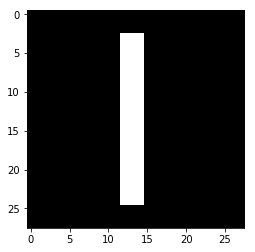
\includegraphics[width=0.2\textwidth]{vertical.png}} *
\begin{pmatrix}
    0 & 0 & 0\\
    0 & 1 & 0\\
    0 & 0 & 0
\end{pmatrix} = 
\raisebox{-.5\height}{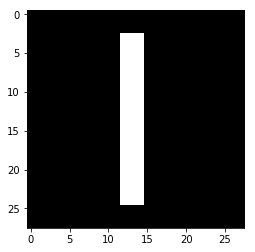
\includegraphics[width=0.2\textwidth]{vertical.png}} 
$$

$$
\raisebox{-.5\height}{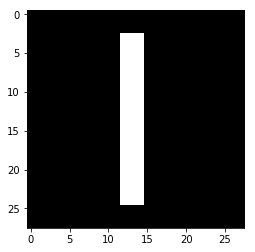
\includegraphics[width=0.2\textwidth]{vertical.png}} *
\begin{pmatrix}
    1 & -1 & 0\\
    0 & 0 & 0\\
    0 & 0 & 0
\end{pmatrix} = 
\raisebox{-.5\height}{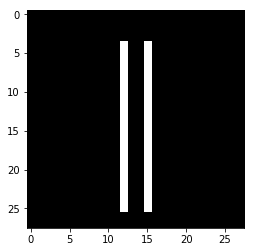
\includegraphics[width=0.2\textwidth]{vx.png}} 
$$
$$
\raisebox{-.5\height}{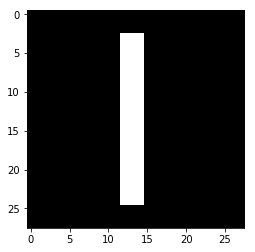
\includegraphics[width=0.2\textwidth]{vertical.png}} *
\begin{pmatrix}
    1 & 0 & 0\\
    -1 & 0 & 0\\
    0 & 0 & 0
\end{pmatrix} = 
\raisebox{-.5\height}{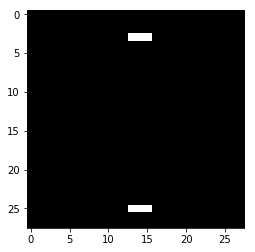
\includegraphics[width=0.2\textwidth]{vy.png}} 
$$
$$
\raisebox{-.5\height}{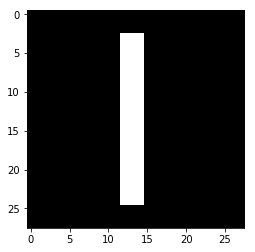
\includegraphics[width=0.2\textwidth]{vertical.png}} *
\begin{pmatrix}
    -1 & 0 & 0\\
    0 & 1 & 0\\
    0 & 0 & 0
\end{pmatrix} = 
\raisebox{-.5\height}{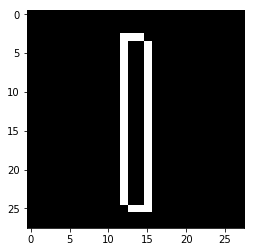
\includegraphics[width=0.2\textwidth]{vxy.png}} 
$$
$$
\raisebox{-.5\height}{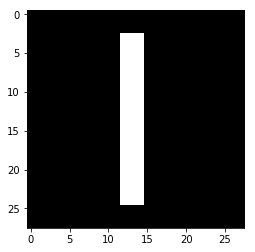
\includegraphics[width=0.2\textwidth]{vertical.png}} *
\begin{pmatrix}
    0 & -1 & 0\\
    -1 & 4 & -1\\
    0 & -1 & 0
\end{pmatrix} = 
\raisebox{-.5\height}{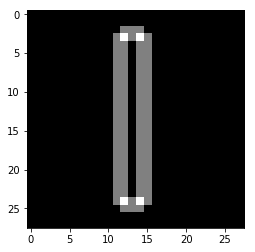
\includegraphics[width=0.2\textwidth]{vlaplace.png}} 
$$

\item A slash bar
$$
\raisebox{-.5\height}{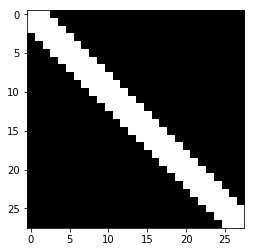
\includegraphics[width=0.2\textwidth]{slash.png}} *
\begin{pmatrix}
    0 & 0 & 0\\
    0 & 1 & 0\\
    0 & 0 & 0
\end{pmatrix} = 
\raisebox{-.5\height}{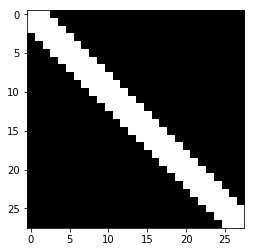
\includegraphics[width=0.2\textwidth]{slash.png}} 
$$

$$
\raisebox{-.5\height}{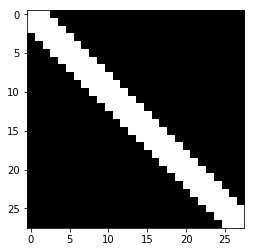
\includegraphics[width=0.2\textwidth]{slash.png}} *
\begin{pmatrix}
    1 & -1 & 0\\
    0 & 0 & 0\\
    0 & 0 & 0
\end{pmatrix} = 
\raisebox{-.5\height}{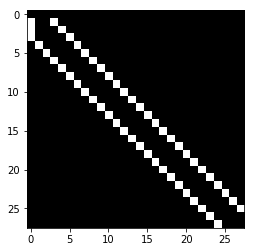
\includegraphics[width=0.2\textwidth]{sx.png}} 
$$
$$
\raisebox{-.5\height}{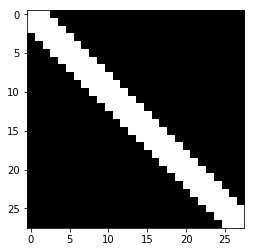
\includegraphics[width=0.2\textwidth]{slash.png}} *
\begin{pmatrix}
    1 & 0 & 0\\
    -1 & 0 & 0\\
    0 & 0 & 0
\end{pmatrix} = 
\raisebox{-.5\height}{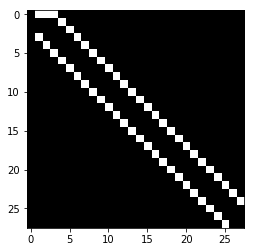
\includegraphics[width=0.2\textwidth]{sy.png}} 
$$
$$
\raisebox{-.5\height}{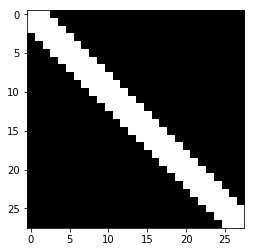
\includegraphics[width=0.2\textwidth]{slash.png}} *
\begin{pmatrix}
    -1 & 0 & 0\\
    0 & 1 & 0\\
    0 & 0 & 0
\end{pmatrix} = 
\raisebox{-.5\height}{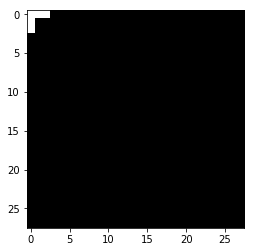
\includegraphics[width=0.2\textwidth]{sxy.png}} 
$$
$$
\raisebox{-.5\height}{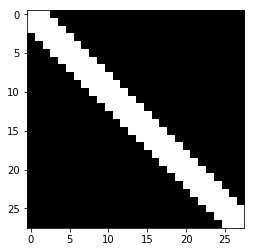
\includegraphics[width=0.2\textwidth]{slash.png}} *
\begin{pmatrix}
    0 & -1 & 0\\
    -1 & 4 & -1\\
    0 & -1 & 0
\end{pmatrix} = 
\raisebox{-.5\height}{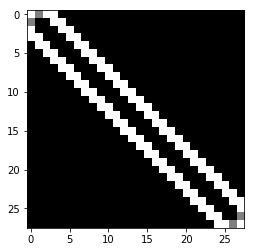
\includegraphics[width=0.2\textwidth]{slaplace.png}} 
$$


\item Identity kernel
$$
\raisebox{-.5\height}{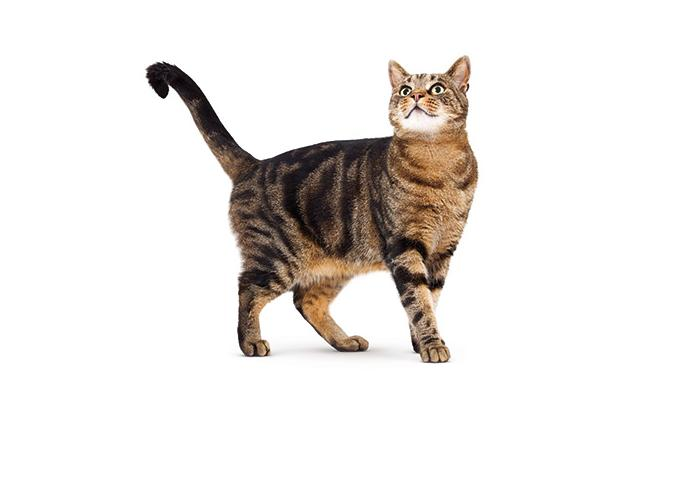
\includegraphics[width=0.2\textwidth]{k0.jpg}} *
\begin{pmatrix}
    0 & 0 & 0\\
    0 & 1 & 0\\
    0 & 0 & 0
\end{pmatrix} = 
\raisebox{-.5\height}{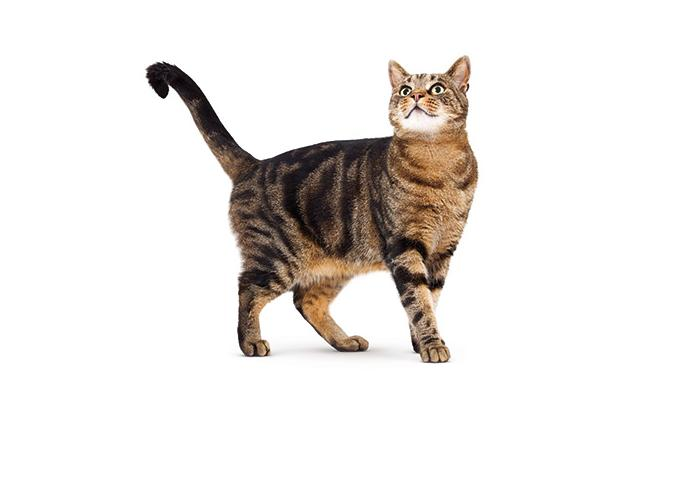
\includegraphics[width=0.2\textwidth]{k0.jpg}} 
$$
\item Kernel that taking $\frac{\partial}{\partial x}$
$$
\raisebox{-.5\height}{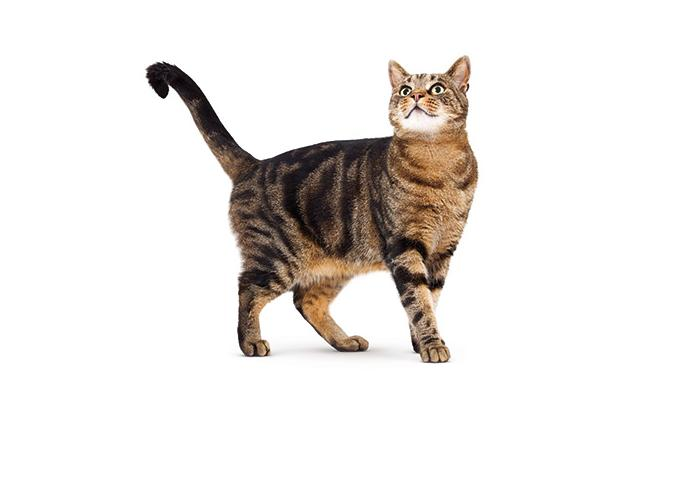
\includegraphics[width=0.2\textwidth]{k0.jpg}} *
\begin{pmatrix}
    1 & -1 & 0\\
    0 & 0 & 0\\
    0 & 0 & 0
\end{pmatrix} = 
\raisebox{-.5\height}{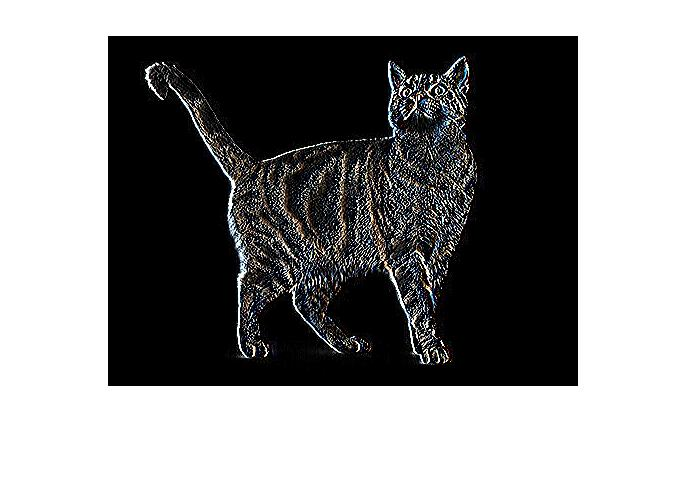
\includegraphics[width=0.2\textwidth]{k1.jpg}} 
$$
\item Kernel that taking $\frac{\partial}{\partial y}$
$$
\raisebox{-.5\height}{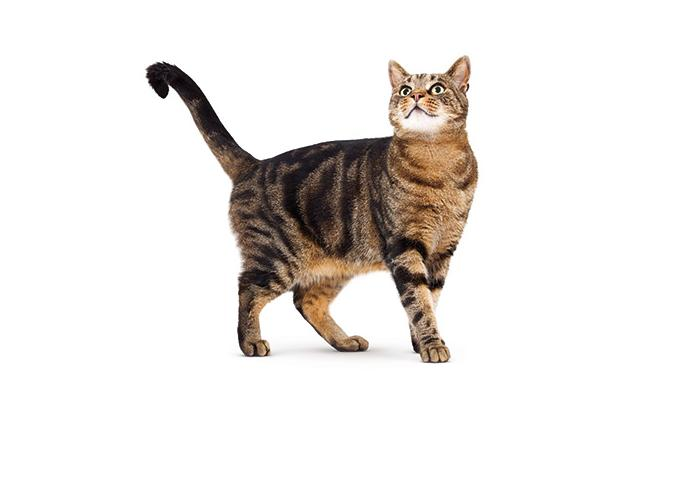
\includegraphics[width=0.2\textwidth]{k0.jpg}} *
\begin{pmatrix}
    1 & 0 & 0\\
    -1 & 0 & 0\\
    0 & 0 & 0
\end{pmatrix} = 
\raisebox{-.5\height}{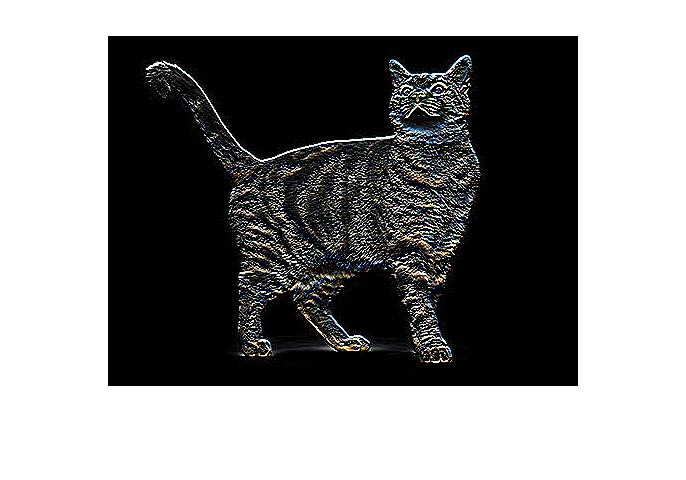
\includegraphics[width=0.2\textwidth]{k2.jpg}} 
$$
\item Kernel that taking $\frac{\partial}{\partial x}+\frac{\partial}{\partial y}$
$$
\raisebox{-.5\height}{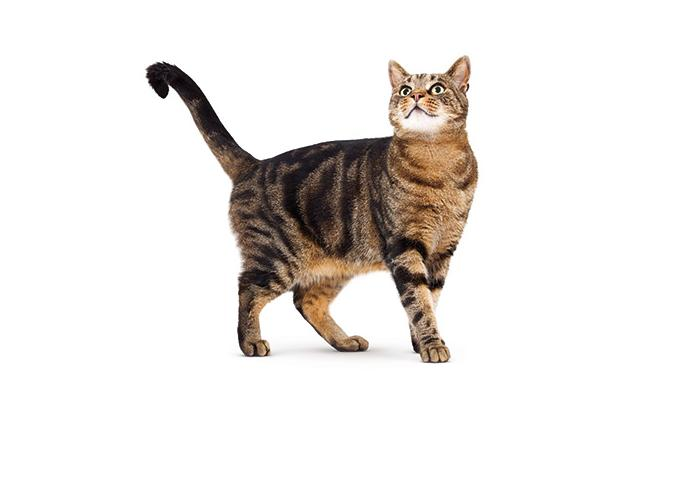
\includegraphics[width=0.2\textwidth]{k0.jpg}} *
\begin{pmatrix}
    1 & 0 & 0\\
    0 & -1 & 0\\
    0 & 0 & 0
\end{pmatrix} = 
\raisebox{-.5\height}{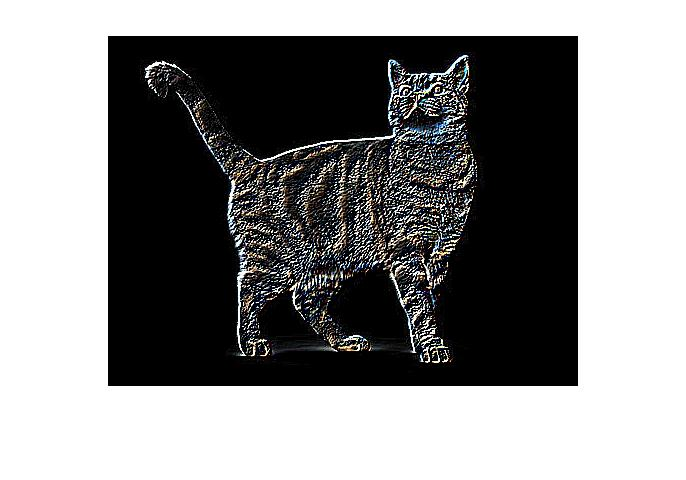
\includegraphics[width=0.2\textwidth]{k3.jpg}} 
$$
\item Kernel that taking $-\Delta$
$$
\raisebox{-.5\height}{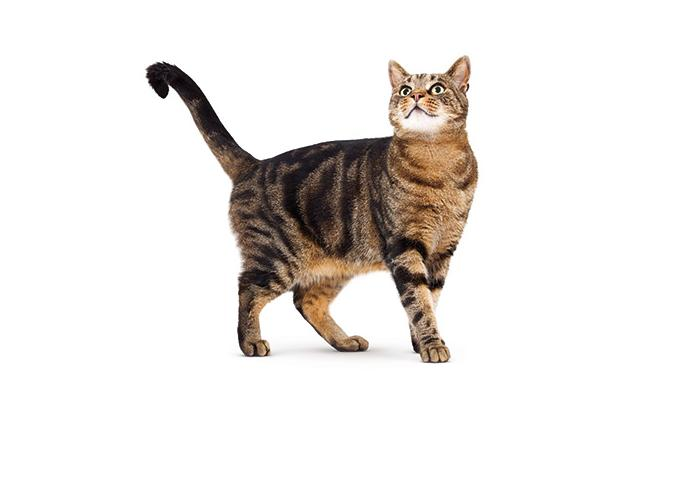
\includegraphics[width=0.2\textwidth]{k0.jpg}} *
\begin{pmatrix}
    0 & -1 & 0\\
    -1 & 4 & -1\\
    0 & -1 & 0
\end{pmatrix} = 
\raisebox{-.5\height}{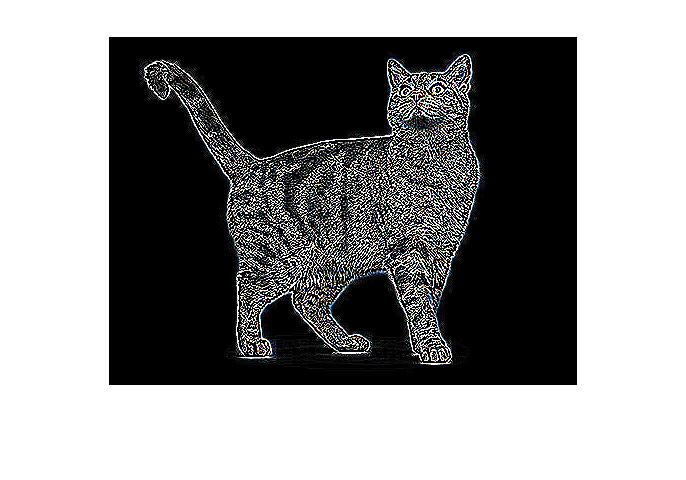
\includegraphics[width=0.2\textwidth]{k4.jpg}} 
$$
\item Kernel that taking local average
$$
\raisebox{-.5\height}{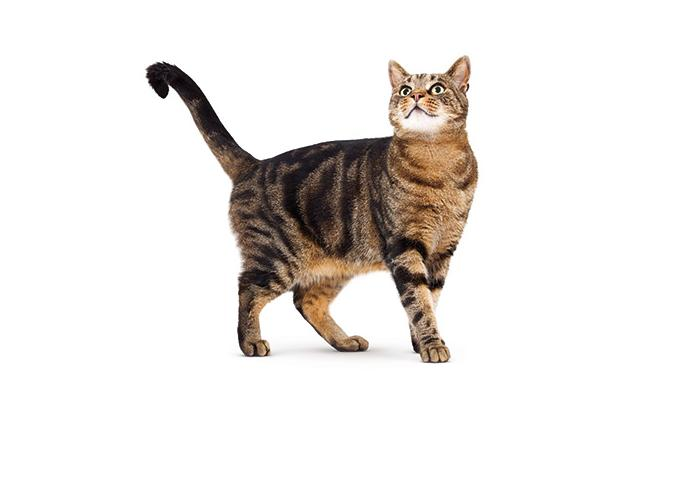
\includegraphics[width=0.2\textwidth]{k0.jpg}} *
\begin{pmatrix}
    1 & 1 & 1\\
    1 & 1 & 1\\
    1 & 1 & 1
\end{pmatrix} = 
\raisebox{-.5\height}{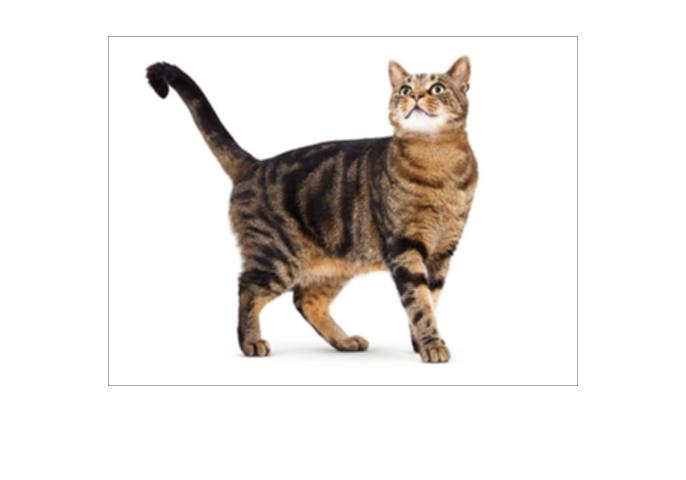
\includegraphics[width=0.2\textwidth]{k5.jpg}} 
$$
\end{itemize}


So if we want to do some AI task like classifier, we cannot only focus on just one feature, so we need many kernels to produce many features. In computer vision, they also call the several channels got from the convolution with different kernels as feature map.  
Because we use more and more kernel after several layers, we need another dimension to denote those several channels, we call this dimension as ``channel dimension". We also have ``essential dimension" w.r.t ``channel dimension" which is the real tensor dimension for this date. For example, for a general colorized picture, is might be $T \in \mathbb{R}^{512\times 512 \times 3}$, here the essential dimension is the first two dimension, and the third one is the $RGB$ channel dimension to represent the colour for picture. 



\subsubsection{Convolution for multichannel case}
Here in real data, we have some special data like colour image $X \in \mathbb{R}^{n \times m \times3}$. Here this image is a 2D graph, with $3$ means the $RGB$ channels. So, we cannot just think $X$ as a general $3$-order tensor. 

We may use this as an example, $X \in \mathbb{R}^{n\times m \times c}$, as we mentioned before, we say that $n \times m$ is the essential dimension and $c$ is the channel dimension for $X$. If we want to do convolution for $X$, here we cannot just use $K \in \mathbb{R}^{2k+1 \times 2k+1}$ because of multichannel. A simple idea is to use also different $c$ kernels and collect them together as $K \in \mathbb{R}^{2k+1 \times 2k+1 \times c}$, and then we can do the general convolution for signal channel separately. This means that 
\begin{equation}
(X \ast K)_{l} = X_{l}\ast K_{l}.
\end{equation}
But we need to recall that, even for $X \in \mathbb{R}^{n\times m \times c}$ it is in fact only stand for just one 2D image(with multi-channel). So if we talk about features in AI, $(X\ast K) \in \mathbb{R}^{n\times m \times c}$ should be reduced to the essential dimension, one simple way is just to add all the channels value together w.r.t essential dimension(this is equal to added with weights because we can reduce those DoF into the previous $c$ kernels.):
\begin{equation}
(X \hat{\ast} K) = \sum_{l=1}^{c} X_{l}\ast K_{l}. 
\end{equation}
then we have
\begin{equation}
(X \hat{\ast} K) \in \mathbb{R}^{n \times m} \quad \text{with} \quad K \in \mathbb{R}^{2k+1 \times 2k+1 \times c}.
\end{equation}
So, for a given real data with $c$ channels like $X \in  \mathbb{R}^{n\times m \times c}$ if we use kernel $K \in \mathbb{R}^{2k+1 \times 2k+1 \times c}$ we can only get one signal channel output. To get multichannel form $X$, we just need to use $d$ kernels $K \in \mathbb{R}^{2k+1 \times 2k+1 \times c}$, or we say $K \in \mathbb{R}^{2k+1 \times 2k+1 \times c \times b}$, then we have:
\begin{equation}\label{6.6}
(X \tilde{\ast} K)_{g} =  X \hat{\ast} K_{g},
\end{equation}
with 
\begin{equation}
(X \tilde{\ast} K) \in \mathbb{R}^{n \times m \times b} \quad \text{with} \quad K \in \mathbb{R}^{2k+1 \times 2k+1 \times c \times b}.
\end{equation}

In the next section, we set that all tensor is with
multichannel(signal channel is a special case, and we note it as $X
\in \mathbb{R}^{n \times m \times 1}$), and we just use $\ast$ no
longer $\tilde{\ast}$. All for all, the  above convolution for multi-channel tensor can be expressed as:
\begin{equation}\label{6.6}
(X \ast K)_{i,j,g} = \sum_{\bm{l}=1}^{c} \sum_{s, t = -k}^k X_{i + s, j + t,\bm{l}} K_{s,t,\bm{l},g},
\end{equation}
with 
\begin{equation}
(X \ast K) \in \mathbb{R}^{n \times m \times b} \quad \text{and} \quad K \in \mathbb{R}^{2k+1 \times 2k+1 \times c \times b}.
\end{equation}











\section{Three basic layers in CNN}
A typical structure in a convolutional network consists of three layers. In the first layer, it performs several convolutions in parallel to produce a set of linear activations. In the second one, each linear activation is run through a nonlinear activation function, such as the rectified linear(ReLu) activation function. This layer is sometimes called the detector layer. In the third layer, we use a pooling function to modify the output of the layer further.
\subsubsection{Convolutional layers}
Here we set that, all the input for the convolutional layer is just one tensor, which means we need collect all channels as the channel dimension. So, for a general tensor with $\hat{c}$ channels $T \in \mathbb{R}^{n_1 \times n_2 \cdots n_d \times \hat{c}}$, we have $\tilde{c}$ convolutional kernels(filter) $K_i \in \mathbb{R}^{2k+1 \times 2k+1 \cdots 2k+1 \times \hat{c}}$ to map it to a $n_1 \times \cdots \times n_d $ tensor with $\tilde c$ channels(feature mapping). 

Mathematically speaking:
\begin{equation}
\ast K_{i}: \mathbb{R}^{n_1 \times n_2 \cdots n_d \times \hat{c}} \xrightarrow{K_i} \mathbb{R}^{n_1 \times  \cdots n_d } \quad \forall i = 1:\tilde c,
\end{equation}
or like the next figure for the ``original convolution with stride 1 for CNN":
\begin{figure}[!htb]        
	\center{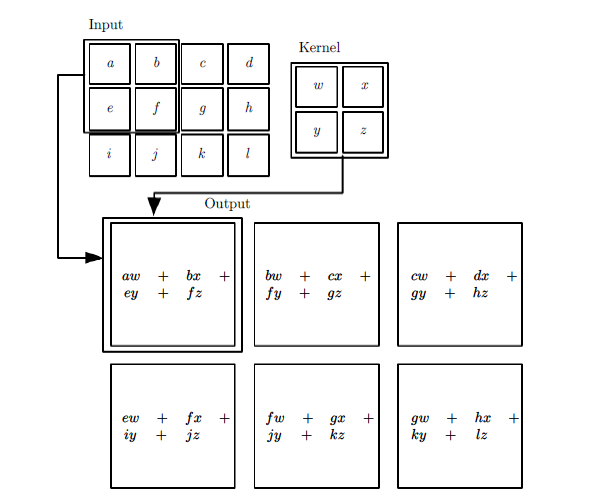
\includegraphics[width=10cm] {Convolution_layer.png}}        
	\caption{An example of 2-D convolution mapping a $3 \times 4$ tensor to a $2 \times 3$ tensor with a convolutional kernal of the size $ 2 \times 2 \times 1$}      
\end{figure}

Generally speaking, $\tilde c \approx 2\hat{c}$, which means this output tensor will become longer in the channel dimension but just a little thinner in the essential dimension. We will introduce ``Pooling'' layers at last, which will keep the channel dimension but reduce the essential dimension very quickly. 

\subsubsection{Nonlinear Activation layers}
This layer is very simple just like the nonlinear layers in feedforward fully connected neural network, just use some simple nonlinear $g: \mathbb{R} \to \mathbb{R}$, such as:
\begin{itemize}
\item Sigmoid or Tangent:
\begin{equation}
g = \sigma (x) = \frac{1}{1 + e^{-x}},
\end{equation}
or 
\begin{equation}
g = tanh(x) = \frac{e^x - e^{-x}}{e^x + e^{-x}}.
\end{equation}

\item Softplus:
\begin{equation}
g(x) = \zeta(x) = \log(1 + \exp{x}).
\end{equation}

\item Rectified Linear Units:
\begin{equation}
g(x) = ReLU(x) = \max\{0,x\}.
\end{equation}
ReLU function is the most commonly used one in nonlinear layers in CNN. 
\end{itemize}


%Then the nonlinear layers can be expressed as:
%\begin{equation}
%f_{ReLu}: \mathbb{R}^{n_1 \times \cdots \times n_d \times \hat{c}} \xrightarrow{ReLU} \mathbb{R}^{n_1 \times  \cdots \times n_d \times \hat{c}}, 
%\end{equation}
%where
%\begin{equation}
%f_{ReLU}(T)(i_1,i_2,\cdots,i_d,i) = ReLU(T(i_1,i_2,\cdots,i_d,i)).
%\end{equation}

\subsubsection{Pooling layers}
For general DNN method, the convolutional layer stands for the linear transformation and then we use a nonlinear layer.  So we just need to repeat this two layers and get a DNN structure.  However, the biggest distinguish between CNN and DNN is the next layer in some degree. 

Just as we mentioned before, the channel dimension will increase twice after a convolution layer but the essential dimension keeps for convolution with padding or only decrease linearly. Another big problem is that, because of the sparsity structure, it is hard to capture some "globally structure" or we see that, this model without some multi-scale structure like in image processing.
 So just as what we do in multigrid method, we need put those fine feature into some coarse level, that is exact the pooling or subsampling in image processing. 

A pooling function is a little like the GMG coarse strategy.   For example, for the output of nonlinear layers with essential order $2$, for one channel $T$, we introduce the pooling method apply to every channel separately: 
\begin{equation}
R(T)_{i,j} = r(T_{2i-1:2i,2j-1:2j})
\end{equation}
$r(\bm{x})$ can be:
\begin{itemize}
\item Fix position: $r(\bm{x}) = x_i$ for some fix $i$. This method can be combine into the convolution with stride as shown before.
\item Maxout: $r(\bm{x}) = \max \{x_1, \cdots, x_4\}$,
\item Average: $r(\bm{x}) = \frac{\sum_{i=1}^4 x_i}{4}$,
\item $L^2$ normal: $r(\bm{x}) = \|x\|$,
\item $\cdots$
\end{itemize}

In computer vision, they think that pooling helps to make the representation become approximately invariant to small translations of the input. Invariance means that if we translate the input by a small amount, the values of most of the pooled outputs do not change.
In each step, with the pooling function, we can transfer the $\tilde c$ channels into $\tilde c$ pooled channels (feature mapping)  separately. 


\section{LeNet-5: The Pioneer of Convolutional Neural Networks}
This section is devoted to a model that is widely recognized as the first convolutional neural network: LeNet-5 \cite{Lecun1998Gradient}. In this section, we will introduce convolutional neural network via introducing LeNet-5 by explain every steps for LeNet-5.
Figure \ref{LeNet-5} shows an illustration of the architecture of LeNet-5. It consists of two pairs of Convolutional Layer and Subsampling Layer and is further connected with fully connected layer and an RBF layer for classification.


\begin{figure}[!htb]
	\center{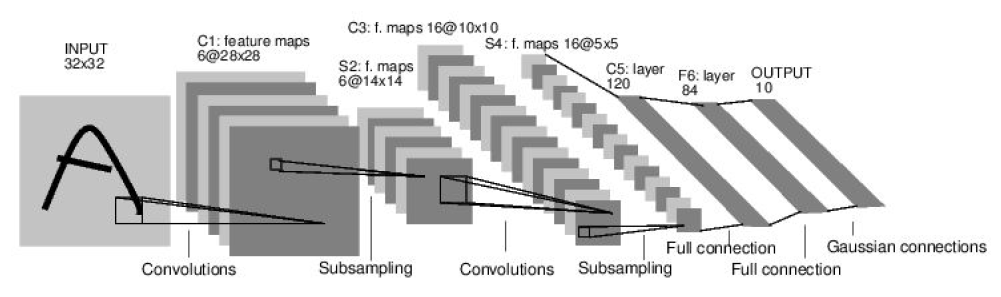
\includegraphics[width=10cm] {LeNet-5.png}}        
	\caption{The Architecture of LeNet-5}      
	\label{LeNet-5}
\end{figure}
%\begin{figure}[htb]        
%	\center{\includegraphics[width=10cm] {AlexNet.png}}        
%	\caption{AlexNet}      
%\end{figure}

\begin{itemize}
\item First of all, the input for LeNet-5 is digital picture with size $32 \times 32$ which every picture contains a number written by different writers. So, mathematically speaking, $T^j$ is a order 2 tensor with just one channel, with essential size $32 \times 32$, i.e $T^j \in \mathbb{R}^{32 \times 32 \times 1}$.  And the out put is a 10-dimensional vector $\bm y = (y_0, \cdots, y_9)$ with $y_i$ equal to the probability for the number in $T^j$ is $i$. 

\item Input: $T \in  \mathbb{R}^{32 \times 32 \times 1}$

\item Input $\xrightarrow{\text{Convolution + ReLU}} C_1$: \\
This layer is not difficult to understand, this means you first use $6$ kernel $K_{1,i}, i = 1:6$ with $K_{1,i} \in  \mathbb{R}^{5 \times 5 \times 1}$, so you get $T\ast K_{1,i}$, and then you just need to use ReLU for $T \ast K_{1,i}, i=1:6$. This means:
\begin{equation}
\mathbb{R}^{32 \times 32 \times 1}  \xrightarrow{\text{Convolution ($K_{1,i}$) + ReLU}} \mathbb{R}^{28\times 28 \times 6} 
\end{equation}
and
\begin{equation}
C_1 = ReLU(T\ast K_{1,i}) \quad i = 1:6.
\end{equation}

\item $C_1 \xrightarrow{\text{Subsampling(Pooling)}} S_2$: \\
This layer is general pooling layer only for essential dimension such as max pooling, average or $L^2$ norm. So we have:
\begin{equation}
\mathbb{R}^{28\times 28 \times 6} \xrightarrow{\text{Pooling}} \mathbb{R}^{14\times 14 \times 6}
\end{equation}

\item $S_2 \xrightarrow{\text{Convolution + ReLU}} C_3$:\\
This layer is a little different form the convolutional layer before because of the fact that $S_2$ is a multi-channel tensor.  So, when we do convolution for them, we need $16$ kernels as $K_{2,i} \in \mathbb{R}^{5 \times 5 \times 6}$:  
\begin{equation}
\mathbb{R}^{14\times 14 \times 6}  \xrightarrow{\text{Convolution ($K_{2,i}$) + ReLU}} \mathbb{R}^{10\times 10 \times 16} 
\end{equation}
and
\begin{equation}
C_3 = ReLU(S_2\ast K_{2,i}) \quad i = 1:16.
\end{equation}
There is an interesting structure for $K_{2,i}$ in the real LeNet-5. That is in the channel dimension for $K_{2,i}$ have some special "0" pattern, which can be shown as:
\begin{figure}[!htb]\label{LeNet-Channel}
	\center{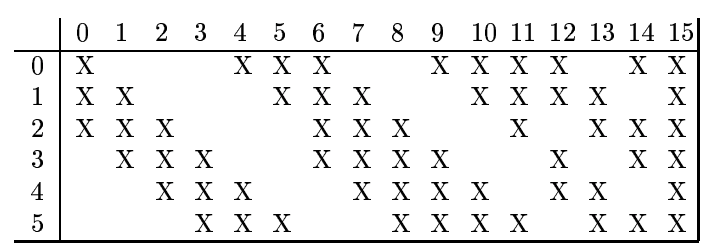
\includegraphics[width=10cm] {LeNet-Channel.png}}        
	\caption{The "0" Pattern for Channel Dimension of $K_{2,i}$}      
\end{figure}

\item $C_3 \xrightarrow{\text{Subsampling(Pooling)}} S_4$:  \\
This layer is the same with $C_1 \xrightarrow{\text{Subsampling(Pooling)}} S_2$. 

\item $S_4 \xrightarrow{\text{Subsampling(Pooling)}} C_5$:  \\
This layer use the naive idea we introduced at the beginning that we just reshape the $16$-channels $5\times 5$ tensor into a vector with dimension $400$. And then followed a fully connected feedforward neural network as a classifier.
\end{itemize}


